\subsection{Room Style Clustering}

% \begin{enumerate}
%     \item Information on the user studies and how we develop the clusters.
%     \item collected data through 2 user studies
%     \item transformed the data into 5 datasets
%     \item data reduction through PCA and T-SNE. Cluster with K-means, K-Medoids, agglomerative clustering and DBSCAN. Evalulated through internal indices (silhouette index, DB index, and CH-index) 
% \end{enumerate}

\begin{figure*}[ht!]
\centerline{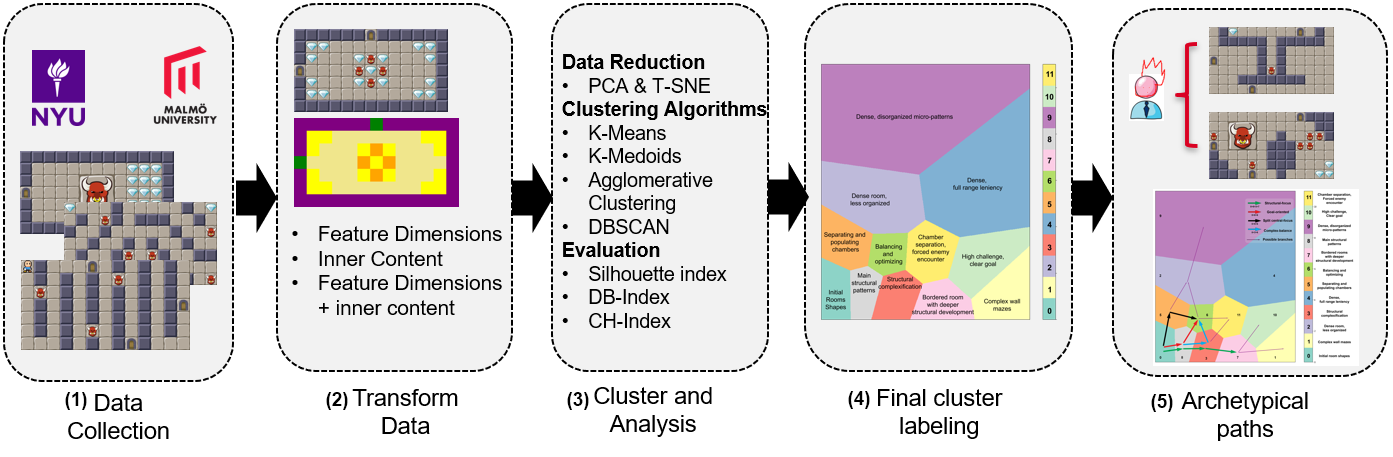
\includegraphics[width=\textwidth]{figures/process-steps.png}}
\caption{The stages of the design style clustering development: (1) Data was first collected through two user studies. (2) Then, using the design sequences, the data was processed into five different datasets, one using the room images, a second using the tiles information, and three using tabular information. (3) A data reduction technique was applied to different datasets, and then they were clustered and internally evaluated. (4) The clusters were formed, picked from the best performing methods, and labeled based on the data points within each cluster. The cluster were evaluated by visualizing how a typical design session traverse the various clusters, and K-Means (K=12) was chosen as the final approach. (5) Finally, using this final approach all the sequences were clustered and archetypical paths were identified.%(5) The final approach,  K-Means (K=12) was evaluated by visualizing how a typical design session traverse the various clusters. Finally, the sequences were clustered by the final approach and archetypical paths were identified.
} \label{p6fig:approach-steps}
\end{figure*}

\begin{figure*}[t]
\centerline{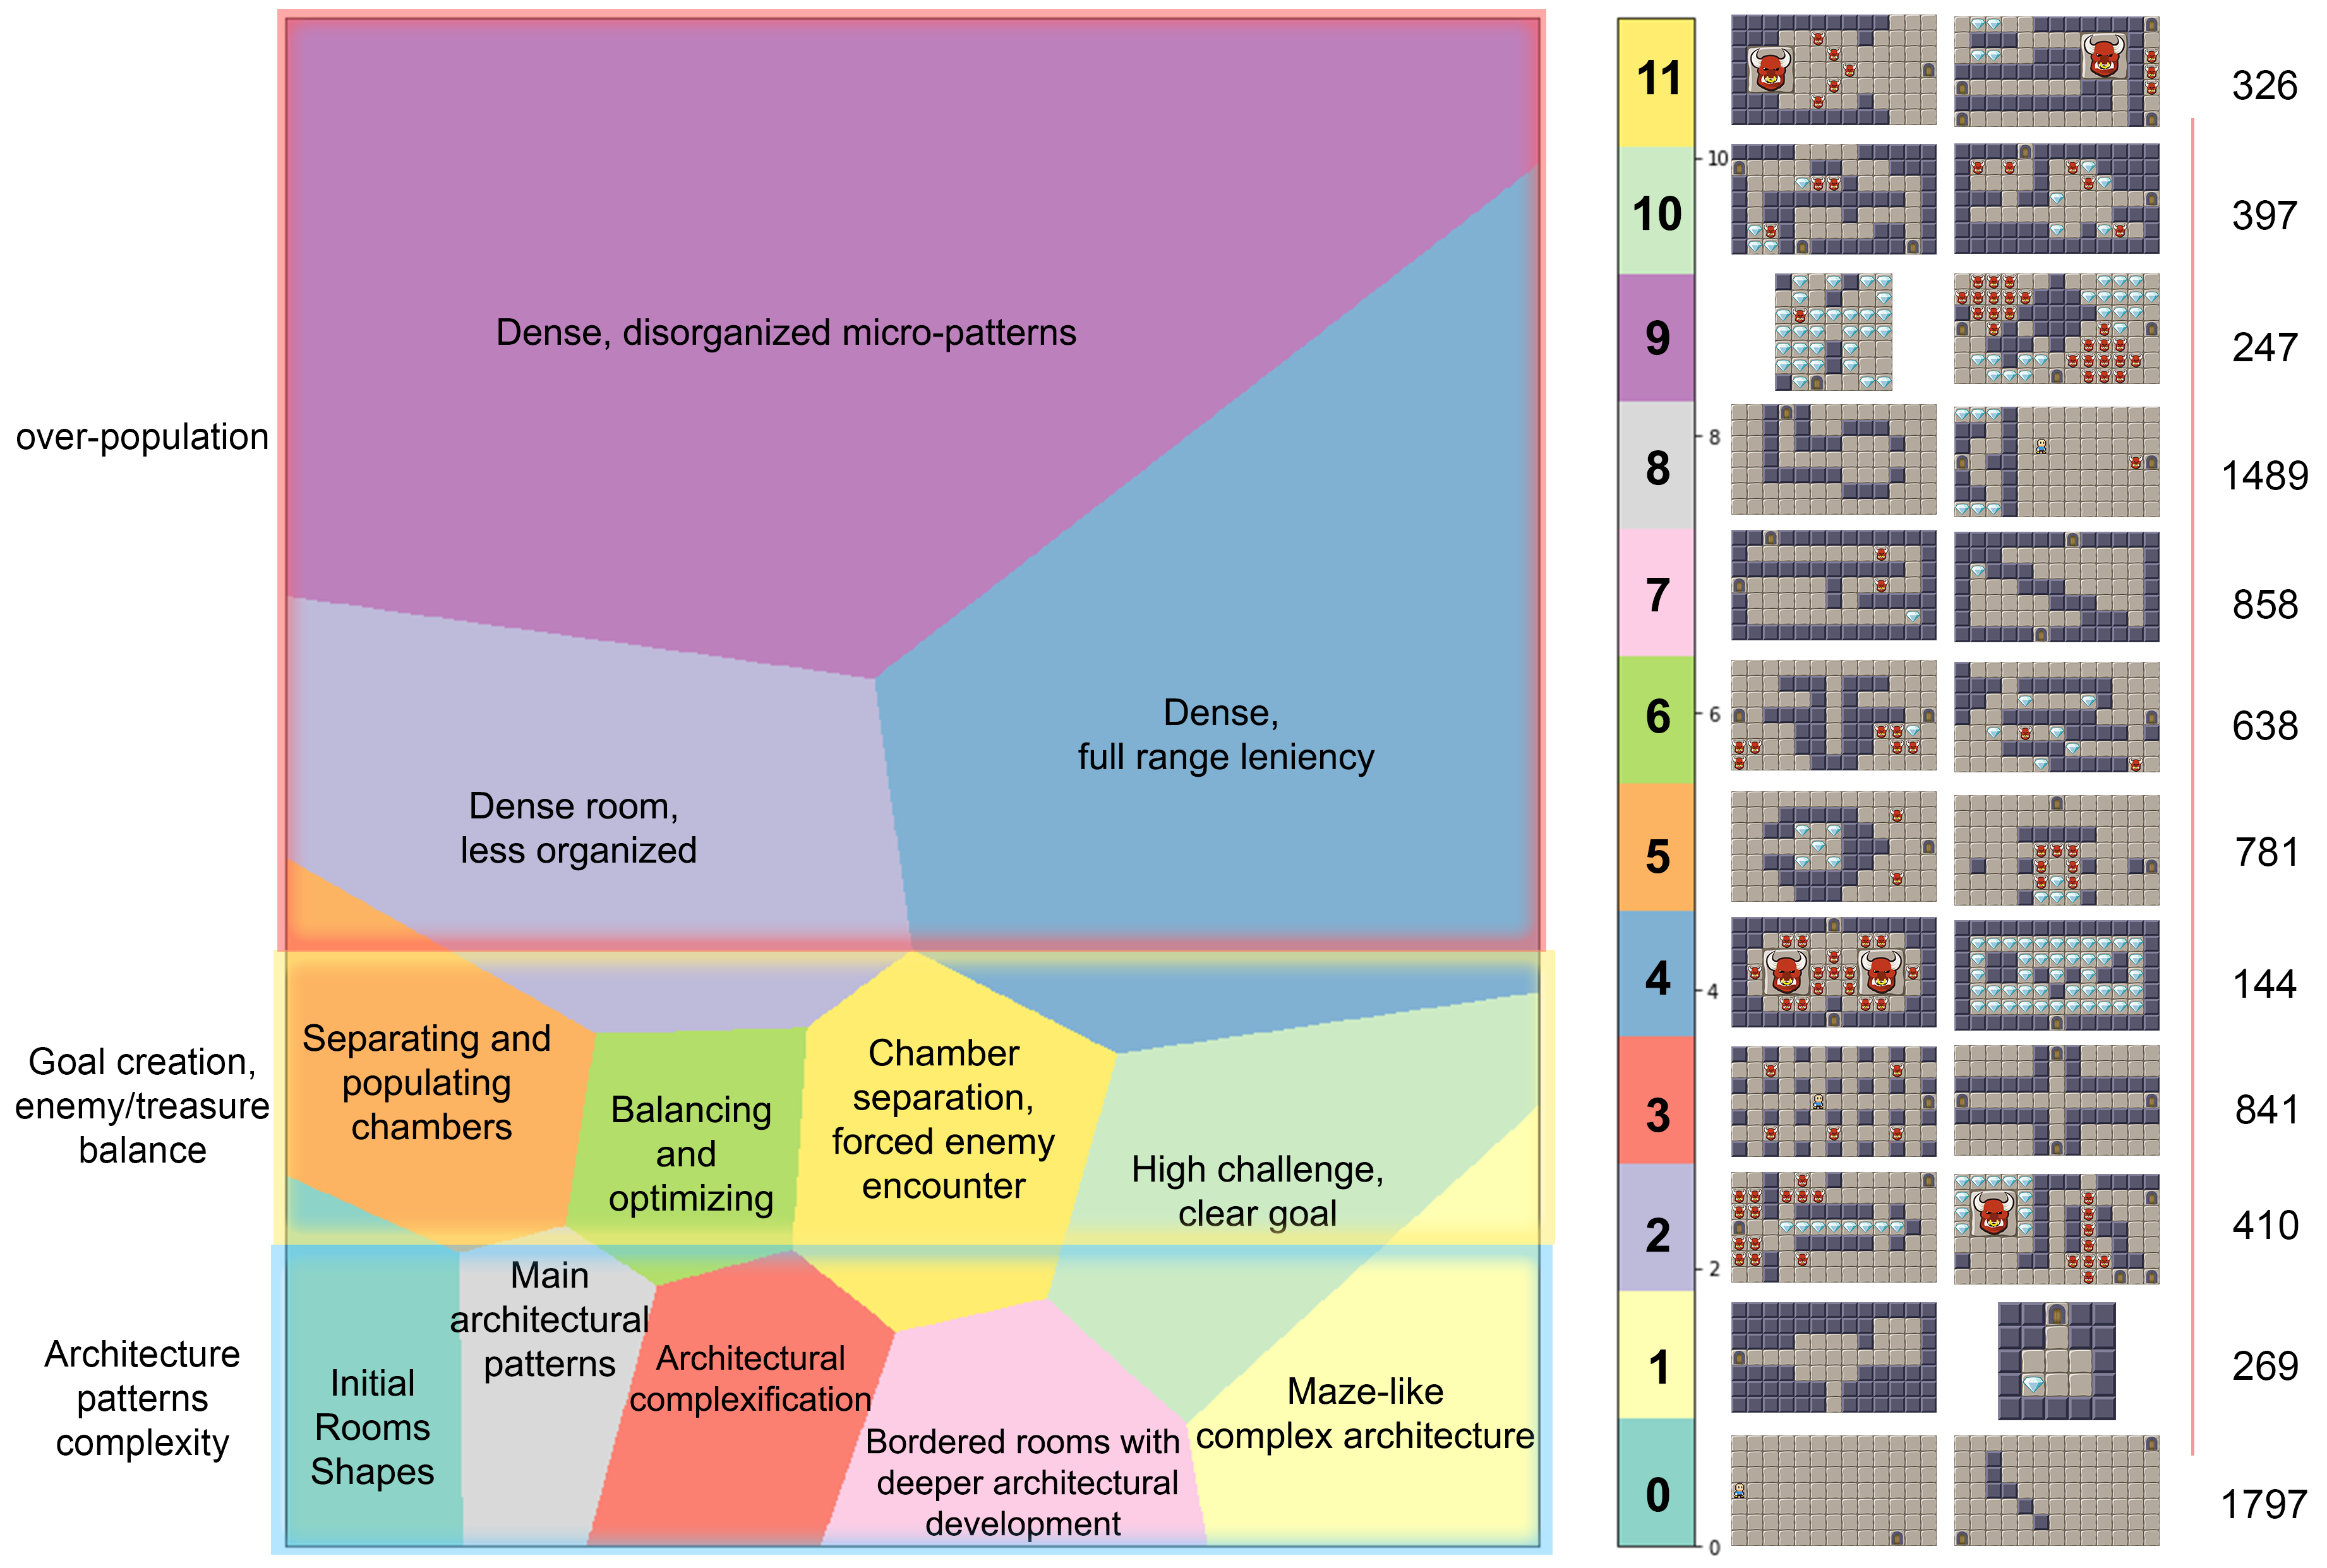
\includegraphics[width=\textwidth]{figures/final-cluster.png}}
\caption{Best resulting cluster set. K-Means (K=12), using the \textbf{Tiles} Dataset. While it scores slightly less in the internal indices that other setups, a qualitative analysis successfully gives us more granularity by subdividing the main bottom clusters, to label and cluster the design process of designers. Sample rooms belonging to each cluster are displayed on the right, next to the total number of rooms in the cluster.} \label{p6fig:all-clusters}
\end{figure*}

% \begin{figure*}[b]
% \centerline{\includegraphics[width=13cm]{figures/representative cluster-steps.png}}
% \caption{Examples of a step by step edition sequence of a design session and it's clustering. To the left, we present the actual sequence and steps of one of the rooms in the dataset and to the right is the actual trajectory of the design in the cluster space. Numbered and in black, it is shown how each step of the design process is clustered by our approach} \label{p6fig:paths-designers}
% \end{figure*}

% \begin{figure}[h]
% \centerline{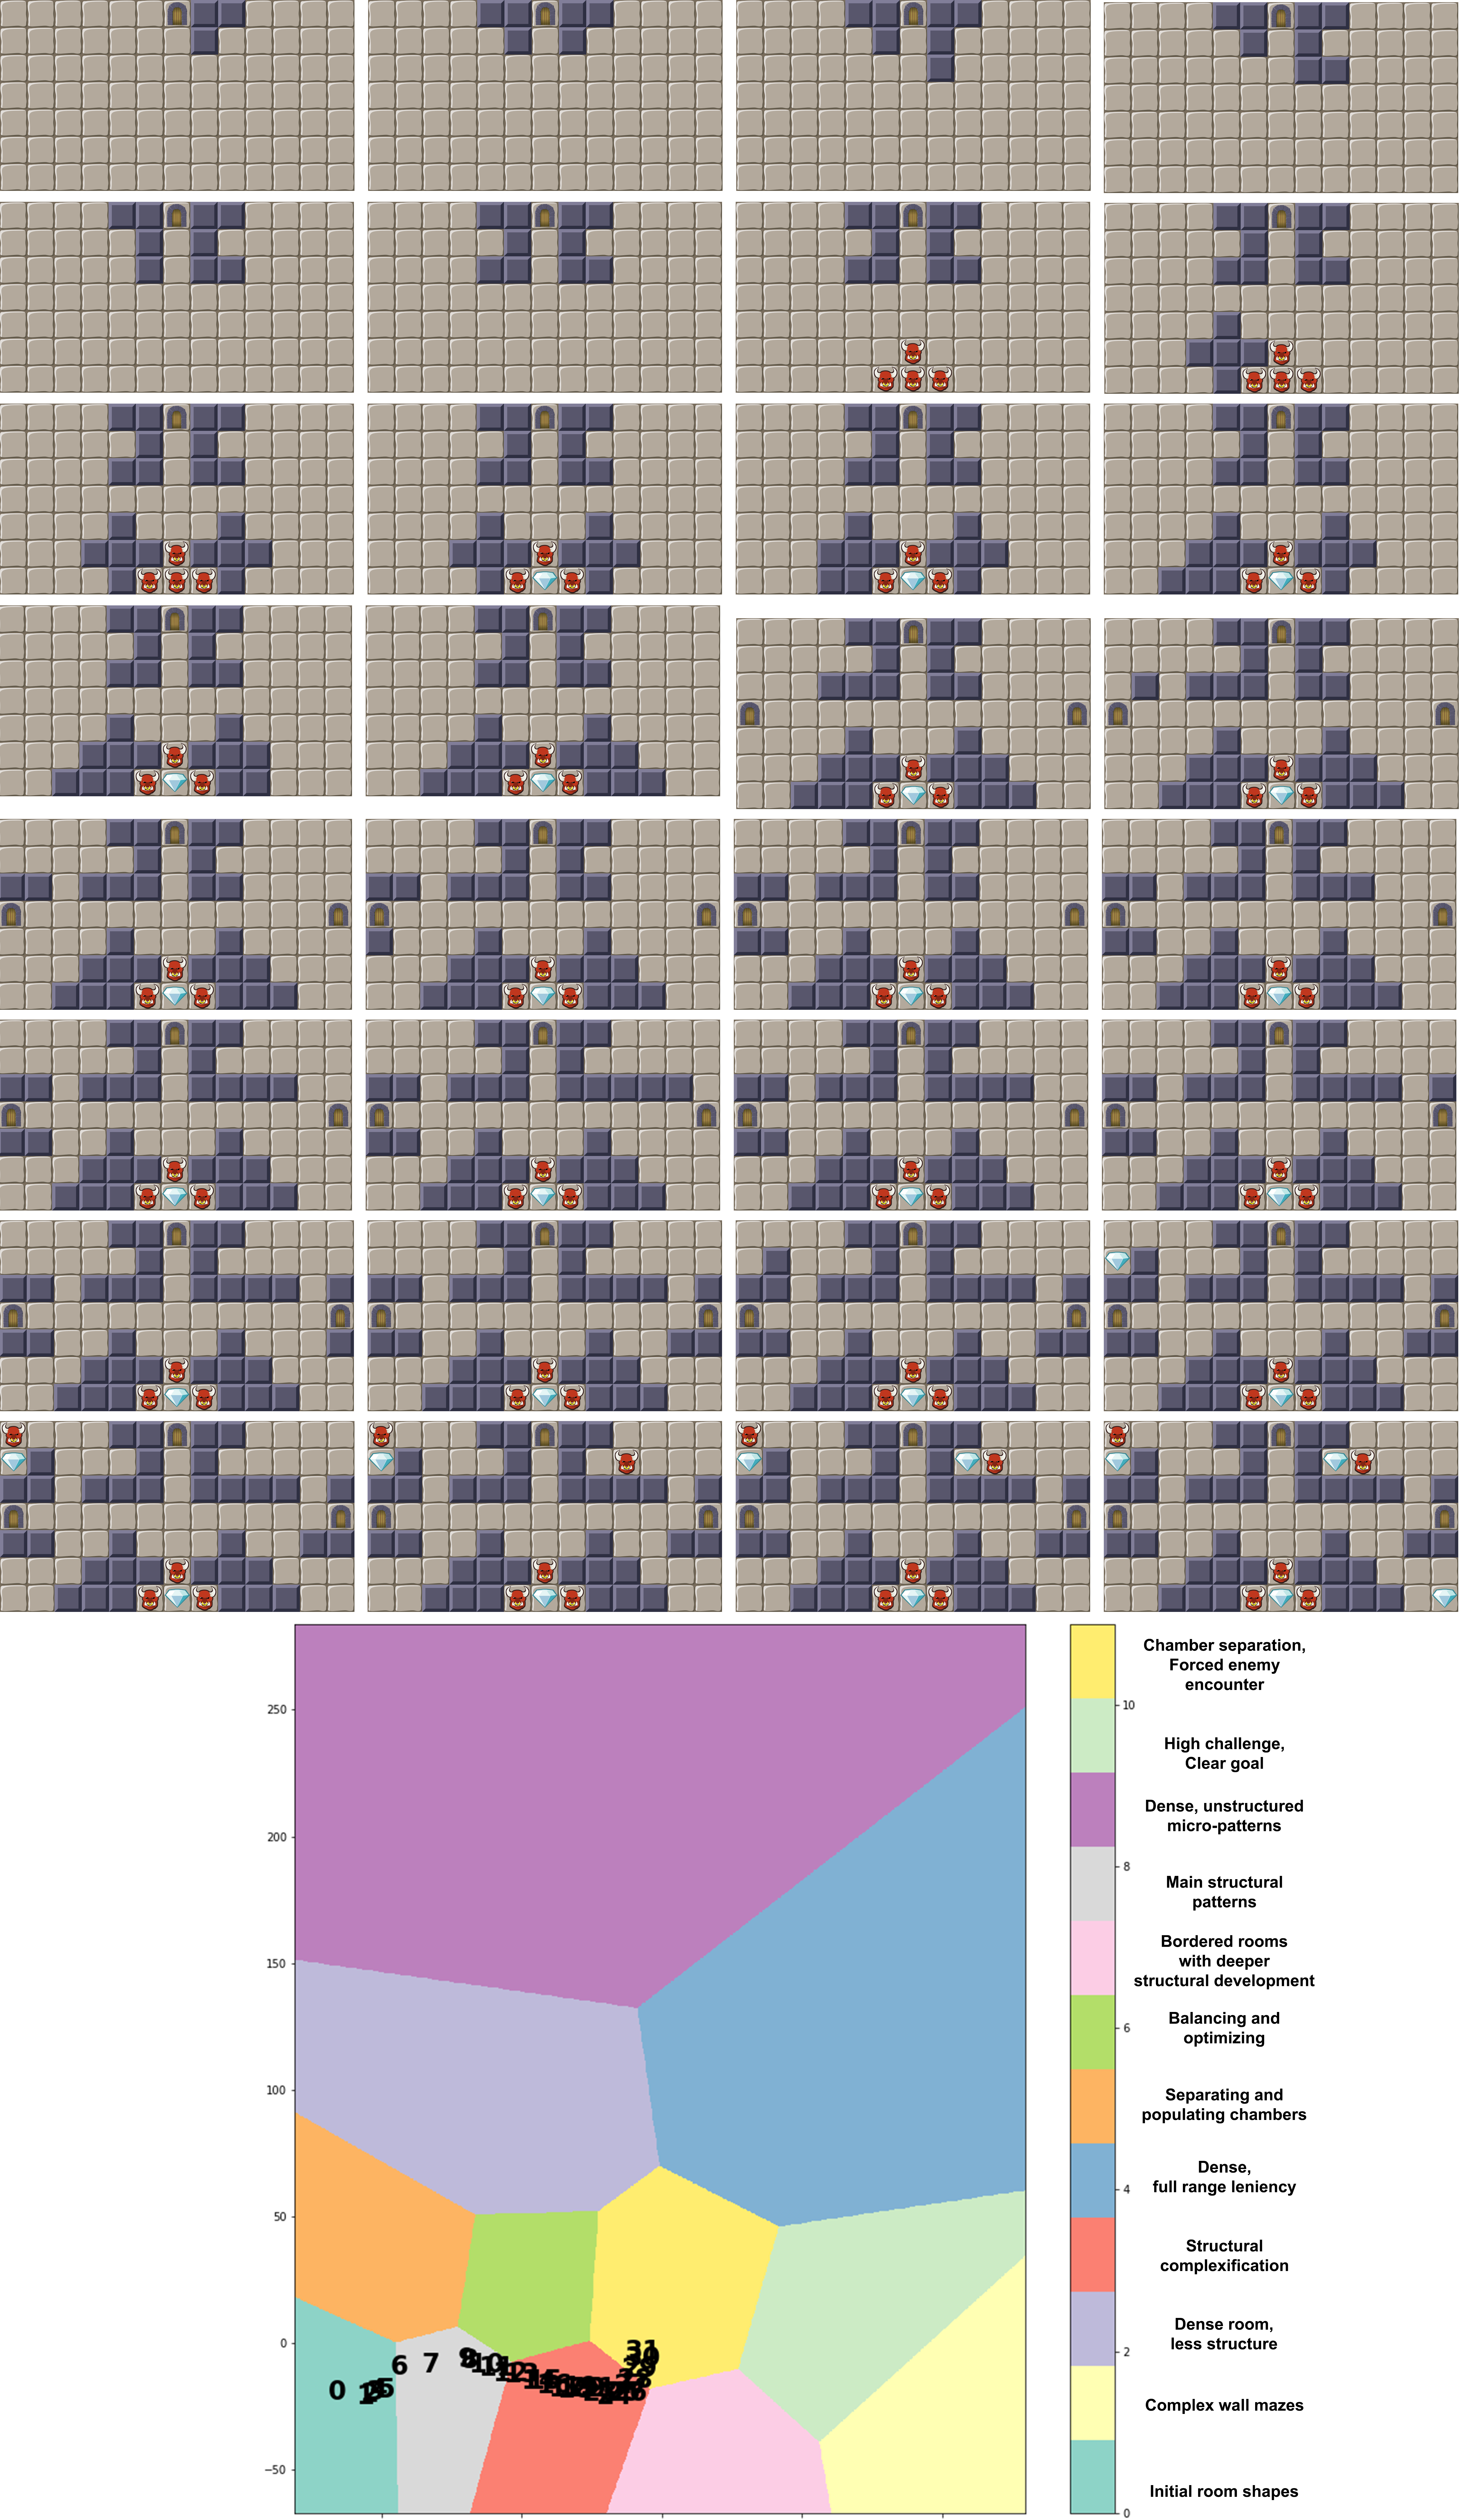
\includegraphics[width=8cm]{figures/representative-cluster-steps-alter.png}}
% \caption{Example of a step by step edition sequence of a design session and it's clustering. At the top, we present the actual sequence and steps of one of the rooms in the dataset, in a $4\times7$ grid, starting at the top left with the first edition. At the bottom, it is the actual trajectory of the design in the cluster space. Numbered and in black, it is shown how each step of the design process is clustered by our approach} \label{p6fig:paths-designers}
% \end{figure}

\begin{figure*}
\centerline{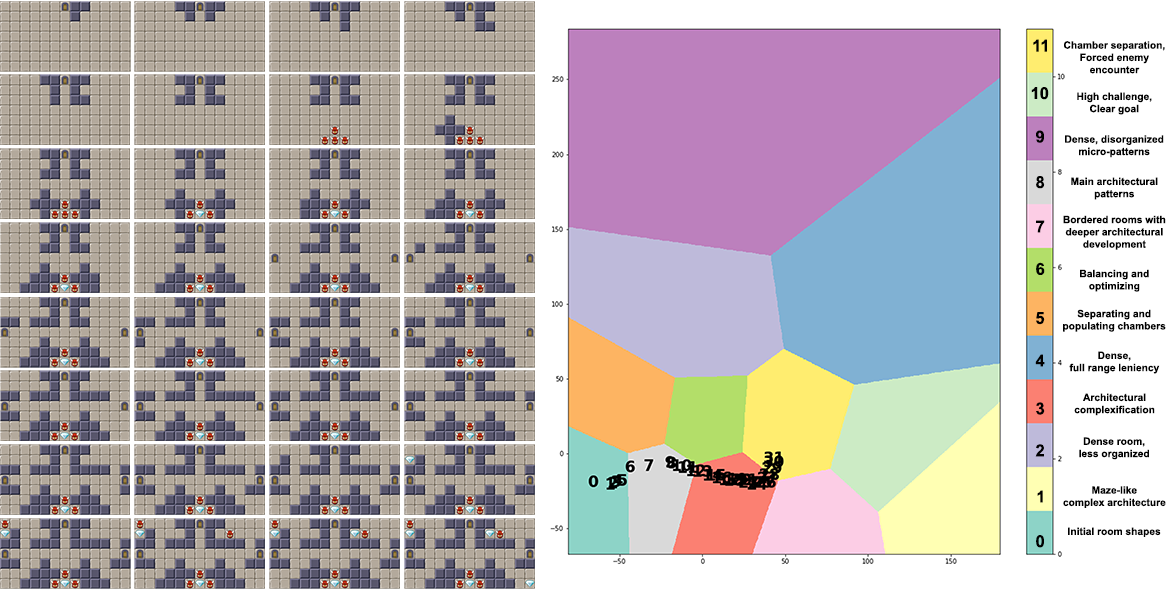
\includegraphics[width=\textwidth]{figures/representative-clusters-small.png}}
\caption{Example of a step by step edition sequence of a design session and it's clustering. At the left, we present the actual sequence and steps of one of the rooms in the dataset, in a $4\times7$ grid, starting at the top left with the first edition. At the bottom, it is the actual trajectory of the design in the cluster space. Numbered and in black, it is shown how each step of the design process is clustered by our approach} \label{p6fig:paths-designers}
\end{figure*}

This paper presents an approach and fundamental steps towards the implementation of designer personas: an analysis of designer style clustering to isolate archetypical paths that can be later be used to build ML surrogate models of archetypal designers. Such models would adapt to the dynamic designer during the mixed-initiative creative process by being placed in the solution space, allowing the designer to traverse such space of models as she drifts through the many dimensions of her creative process.

The proposed system builds on top of EDD's Designer Preference Model and preliminary results \citepsixth{p6Alvarez2020-DesignerPreference}, expanding it to classify the designers' designs based on clusters developed using previously hand-made design sequences by expert and non-expert designers. Figure \ref{p6fig:approach-steps} illustrates our approach in five sequential stages, from data collection to experimentation and results. The first four stages are explained in the following subsections, whereas Section~\ref{p6section:results} shows the experimental results.

\subsubsection{Data Collection}

We conducted two user studies where participants were tasked with freely designing a dungeon in EDD and the rooms that compose it with no further restrictions, using all the available tiles i.e. floor, wall, treasure, enemy, and boss tiles. All participants were introduced to the tool before the design exercise. User-generated data was gathered during the complete design session, creating a new data entry every time the designer edited the dungeon. In total, we had $40$ participants, $25$ of these (i.e. NYU participants) were industry or academic researchers within the Games and AI field, and the other $15$ (i.e. MAU participants) were game design students. This resulted in a diverse dataset composed of $180$ unique rooms like the ones depicted in Figure~\ref{p6fig:approach-steps}, that was pre-processed and clustered in the subsequent stages. 

\subsubsection{Dataset pre-processing}

From the $180$ unique rooms, we extracted and used the edition sequence of each of the rooms, from their initial design to the more elaborated end-design, to compose a richer dataset that could capture the design process of a designer rather than focusing on the end-point. Through this, we ended up using $8196$ data points in our dataset.
%just the end-point. We ended up using $8196$ rooms
Moreover, five different copies of the dataset were created to analyze and compare the performance of the clustering stage using the following image pre-processing methods:

\begin{enumerate}
\setcounter{enumi}{0}
    \item \textbf{Room:} No pre-processing. Room images are fed into the next stage as they were created by the designer, with a resolution of $1300\times 700\times3$, corresponding to width, height, and RGB ($3$ color channels).
    
    \item \textbf{Tiles:} Each room tile type is mapped to a single-color pixel and the rooms are simplified to a pixel-tile based representation, as shown in the second stage of Figure \ref{p6fig:approach-steps}. The dimensions are downscaled to $13\times 7\times3$.
    %Each room tile is simplified to a single-color pixel, as shown in the second stage of Figure \ref{p6fig:approach-steps}, downscaled to $13\times 7\times3$.
    
    \item \textbf{Dimensions:} Each room is described by its five IC-MAP-Elites feature dimension values, excluding the similarity scores: \textsc{Linearity}, \textsc{Leniency}, \textsc{\#MesoPatterns}, \textsc{\#SpatialPatterns}, and \textsc{Symmetry}. A complete description of these features can be found in~\citepsixth{p6Alvarez2020-ICMAPE}.
    
    \item \textbf{Inner Content:} Each room is described by $12$ values, related to the count, sparsity, and density of the enemy, treasure, floor, and wall tiles contained in it.
    
    \item \textbf{Combined:} A combination of the \textbf{Dimensions} and \textbf{Inner Content} methods.
\end{enumerate}

\subsubsection{Clustering and Analysis}

To run all setups, data reduction algorithms, clustering algorithms, and do the internal evaluation of the clusters, we used scikit-learn machine learning toolset~\citepsixth{p6scikit-learn}. To obtain the best set of clusters, we ran different setups with the above datasets. The data was reduced to two meaningful dimensions with two different data reduction algorithms, Principal Component Analysis (PCA) and T-Distributed Stochastic Neighbor Embedding (T-SNE). For both data reduction algorithms, we fit the algorithms with each individual dataset, setting to two principal components and in the case of T-SNE using PCA as initializing algorithm, and transforming the data into a new dataset \emph{pca\_dataset} and \emph{tsne\_dataset} per dataset. Each two-dimensional point in the new datasets represents a step in the sequences described above.%Likewise, for the T-SNE, we fit the algorithm with each individual dataset, setting the parameters to two principal components and using PCA as initializing algorithm, and then transformed the data into a new dataset \textit{tsne_dataset} per dataset.

Moreover, all the resulting datasets were then clustered using \textsc{K-Means, K-Medoids, Agglomerative clustering}, and \textsc{DBSCAN}. K-Means was initialized using the standard k-means++ implemented in scikit-learn, which initialize all centroids distant from each other. K-Medoids was initialized similarly, using the standard k-medoids++, and tested using the \emph{cosine}, \emph{euclidean}, and \emph{manhattan} distances. Agglomerative clustering is a hierarchical clustering approach using a bottom-up approach implemented in scikit-learn using four different linkage criteria for comparing data points: \emph{Ward}, \emph{Complete}, \emph{Average}, and \emph{Single}. Finally, DBSCAN cluster points based on density separated by low-density areas; thus, DBSCAN automatically finds $k$ based on two parameters, $\epsilon$ describing the maximum distance between points and \emph{min\_samples} describing the minimum amount of samples within a group to be considered a cluster. K-Means, K-Medoids, and Agglomerative clustering were tested using multiple $K$ values ranging from 3 to 13, and DBSCAN was tested with several $\epsilon$ values ranging from 0.3 to 1.0, and \emph{min\_samples} ranging from 2 to 9.

%, testing with $K$ values ranging from 3 to 13 for the first three ones, and several $\epsilon$ values for DBSCAN.

%testing different minimum distance between data points ($\epsilon$) and the minimum amount of data points within a cluster to be considered a dense region for DBSCAN.

Since we lack a labeled dataset (i.e. ground truth) for cluster validation, we evaluated the results from all setups using the internal indices below, as well as manually inspecting the rooms composing the resulting clusters.

%Since in our approach lacks a labeled dataset (i.e. ground truth) for cluster validation, 

\begin{itemize}
\item \textbf{Silhouette Score:} The Silhouette Score shows how similar a data point is to the cluster it is associated with, through calculating the difference between the $\overline{distance}$ from the point to the points in the nearest cluster and the $\overline{distance}$ to the points in the actual cluster. The value is bounded from -1 to +1, with values closer to +1 indicating a good separation of the clusters, and closer to -1 meaning that some points might belong to another cluster.
\item \textbf{Davies-Bouldin Index:} The DB-index is the ratio between the within-cluster distances and between-clusters distances. With this, we can have an insight into the average similarity of clusters with their closest cluster. The value is bounded from 0 to +1, with values closer to 0 relate to clusters that are farther apart from each other and less dispersed, thus, this index is more crucial when we have more dense representations.
\item \textbf{Calinski-Harabasz Index:} The CH-index is another index related to the density of the clusters and how well separated they are. The score is the ratio between the within-cluster dispersion (compactness) and the between-cluster dispersion (separation). The CH-index is positively unbounded, and the higher the score the better.
\end{itemize}

\subsubsection{Cluster Labelling}

\begin{table}
\begin{center}
{\caption{Best performing setups based on their internal validation and visualization of clustered data points.}\label{p6table:setups}}
\resizebox{0.9\textwidth}{!}{
\begin{tabular}{ccccccc}
\hline
\rule{0pt}{12pt}
Algorithm&Data&K&$\Diamond$&$\Box$&$\bigtriangleup$ 
\\ 
\hline
\\[-6pt]
K-Means & Tiles-PCA & 9 & 0.43 & 0.73 & 9438.233 \\ 
K-Means & Tiles-PCA & 12 & 0.41 & 0.77 & 9436.928 \\
K-Means & Dimensions-PCA & 12 & 0.43 & 0.73 & 7738.343 \\
Agglomerative single & Combined-PCA & 6 & 0.51 & 0.43  & 38.833 \\ 
Agglomerative avg. & Dimensions-PCA & 6 & 0.44 & 0.67 & 3463.567 \\ 
\hline
\\[-6pt]
\multicolumn{6}{l}{$\Diamond$ Silhouette Score\ \
$\Box$ Davies Bouldin Index\ \
$\bigtriangleup$ Calinski-Harabasz Index}
\end{tabular}
}\end{center}
\end{table}

Table~\ref{p6table:setups} shows the best performing setups according to their internal indices scores. The clusters in these setups were manually inspected in order to detect the qualitative features that better define them. 

When using the \textbf{Dimensions} and \textbf{Combined} datasets, the clusters do perform good, if not better, in certain indices than when using the \textbf{Tiles} dataset. However, when analysing the resulting setups, they were missing a clearer relation between the clustered rooms, which was exacerbated when analysing sequences and paths on these setups, where they missed continuity between clusters.

Conversely, given that we are creating tile-based rooms and dungeons, the features were more representative for the \textbf{Tiles} dataset, which when used, generally performed well in the evaluated internal indices, and the produced clusters meaningfully separate the data. Further, as it will be presented in Section \ref{p6section:results}, when clustering sequences and analyzing the cluster path of the designs, there exist a continuity between designs that supports its usability. Figure \ref{p6fig:all-clusters} shows the best-resulting cluster set found among all the experiments run.



% As expected, the \textbf{Tiles} dataset generally performed well in the evaluated internal indices, and the produced clusters meaningfully separated the data.
% better information and were meaningfully group together.  relation each of the features have with 

% As expected, the \textbf{Tiles} representation have good results across the 3 indices, 

% JOSÉ: I leave it here waiting for the final results from Alberto

%Moreover, We noticed that the agglomerative approach results in very specific clusters alongside a quite broad cluster consisting of unrelated data points, regardless of the $K$ used. These setups scored well in the different indices but fail to accurately partition the space in relevant groups.

%Moreover, there are recurrent clusters between the different setups but when using more clusters like in figure~\ref{p6fig:all-clusters} (b), we can have more granularity when partitioning the space, improving the separation of more related data points. In figure~\ref{p6fig:all-clusters}(b) we present several rooms that have been clustered together matching the labeling of the clusters. In the figure, there is a clear correlation between the designs and the labels of their respective cluster, and an interesting continuity between the final clusters.

% In Figure~\ref{p6fig:all-clusters}, we present the final and selected approach for clustering room styles using K-Means (K=12) and the \textbf{Tiles} dataset reduced with the PCA algorithm. To the right, next to each color in the legend, we have different representative rooms that belong to the clusters, in their respective color, and have been clustered together. Furthermore, besides the local relation between clusters, there exists a layered division among group of clusters in the y-axis, where the bottom clusters relate more to architectural pattern complexity, from very empty rooms to mazes. The middle clusters focus on populating the rooms with enemies and treasures, creating the actual goals of the room and balancing the challenge. Finally, the top clusters are composed of dense rooms where the enemy and treasure addition do not necessarily need to follow any clear objective. 


% The clusters's label are plotted on top of each of the clusters, describing in general, the content that is within them. These cluster 

In the figure, we have plotted on top of the clusters the labels describing in general, the content that is within them. The following is a description of the clusters and the rooms that were clustered together:

\textbf{0. Empty-Initial rooms:} %This cluster contains $1797$ data points, and 
This cluster relates mostly to the initial designs made by the designers. These designs are from completely empty rooms to initial work-in-progress structures.

\textbf{1. Maze-like complex architecture:} This cluster to the extreme of the architectural patterns complexity layer, relates to more highly-linear, confined and maze-like rooms.% with more structure on what is possible. %The cluster contains $269$ data points.

\textbf{2. Dense, less organized:} This cluster contains rooms that still have a certain objective but are moving towards more disorganized distributions of micro-patterns in relation to their density. %This cluster contains $410$ data points.

\textbf{3. architectural complexification:} %This cluster contains $841$ data points, and 
This cluster relates mostly to the complexification of wall structures by having dense wall chunks, representative architectural patterns, or symmetrical patterns.

\textbf{4. Dense, full range leniency:} Focusing on density as the other two clusters within the same layer, this cluster relates to rooms that are in the full range of leniency from very rewarding, treasure rooms to very challenging boss rooms. %This cluster contains $144$ data points.

\textbf{5. Separating and populating chambers:} This cluster relates to the process of separating rooms into distinct chambers, focusing on the center of the room, and starting to populate rooms with enemies and treasures. %The cluster contains $781$ data points.

\textbf{6. Balancing and optimizing:} This cluster contains a mix between corridors and chambers within rooms with a focus on balancing rooms and optimizing their design towards certain goals. %The cluster contains $638$ data points.

\textbf{7. Bordered rooms with deeper architectural development:} This cluster relates mostly to rooms with an added wall border by the designer, and where the focus is to shape chambers and develop more visual structures.

\textbf{8. Main architectural shapes:} Similar to other clusters within the same layer, this cluster relates to the development and definition of main architectural patterns that are somewhat symmetric.

\textbf{9. Dense, disorganized micro-patterns:} This cluster clusters the extreme rooms that contain a high density of tiles, other than floor-tiles, without a clear structure or objective for the player.

\textbf{10. High challenge, clear goal:} This cluster relates to well-shaped rooms with clear wall structures and goals, towards more challenge. 

\textbf{11. Chamber separation with forced enemy encounter:} This cluster relates to rooms that are in the process of a clear segmentation into corridors and chambers, and that enforce to some extent, enemy encounters for the player. 

Furthermore, besides the local relation between clusters, the clusters are implicitly divided in three layers on the Y-axis. From bottom to top, (a) architectural patterns complexity, relating to clusters composed of rooms with clearer or complex shapes done with walls, from empty rooms to mazes. (b) Goal creation, enemy/treasure balance, with clusters comprehending the strategic addition of enemies and treasures to establish objectives in the room for the player. In terms of EDD, these rooms are composed of more meso patterns. And (c), over-population, which relates to clusters filled with less organized and dense rooms where the enemy and treasure addition do not necessarily need to follow any clear objective. Identifying the designer in such layer, and the path they have taken to get there could show meaningful information in the design process. For instance, the intentions of the designer, in what phase of the design process she is at the moment i.e. trying the tool or observing how the tool reacts or scraping her current goal towards a new goal within the room. 

% \begin{enumerate}
% \setcounter{enumi}{-1}
% \item[0] \textbf{Empty/Initial rooms:}
% \item \textbf{Complex wall mazes:} 
% \item \textbf{Dense, less structure} 
% \item \textbf{Structural complexification:} 
% \item \textbf{Dense, full range leniency} 
% \item \textbf{Separating and populating chambers:} 
% \item \textbf{Balancing and optimizing rooms:} 
% \item \textbf{Bordered rooms with deeper structural development:}
% \item \textbf{Development of main structural shapes:} 
% \item \textbf{Dense, unstructured:} 
% \item \textbf{Challenging rooms with clear goal:} 
% \item \textbf{Chamber separation with forced enemy encounter:} 
% \end{enumerate}



\begin{figure*}[t!]
\centerline{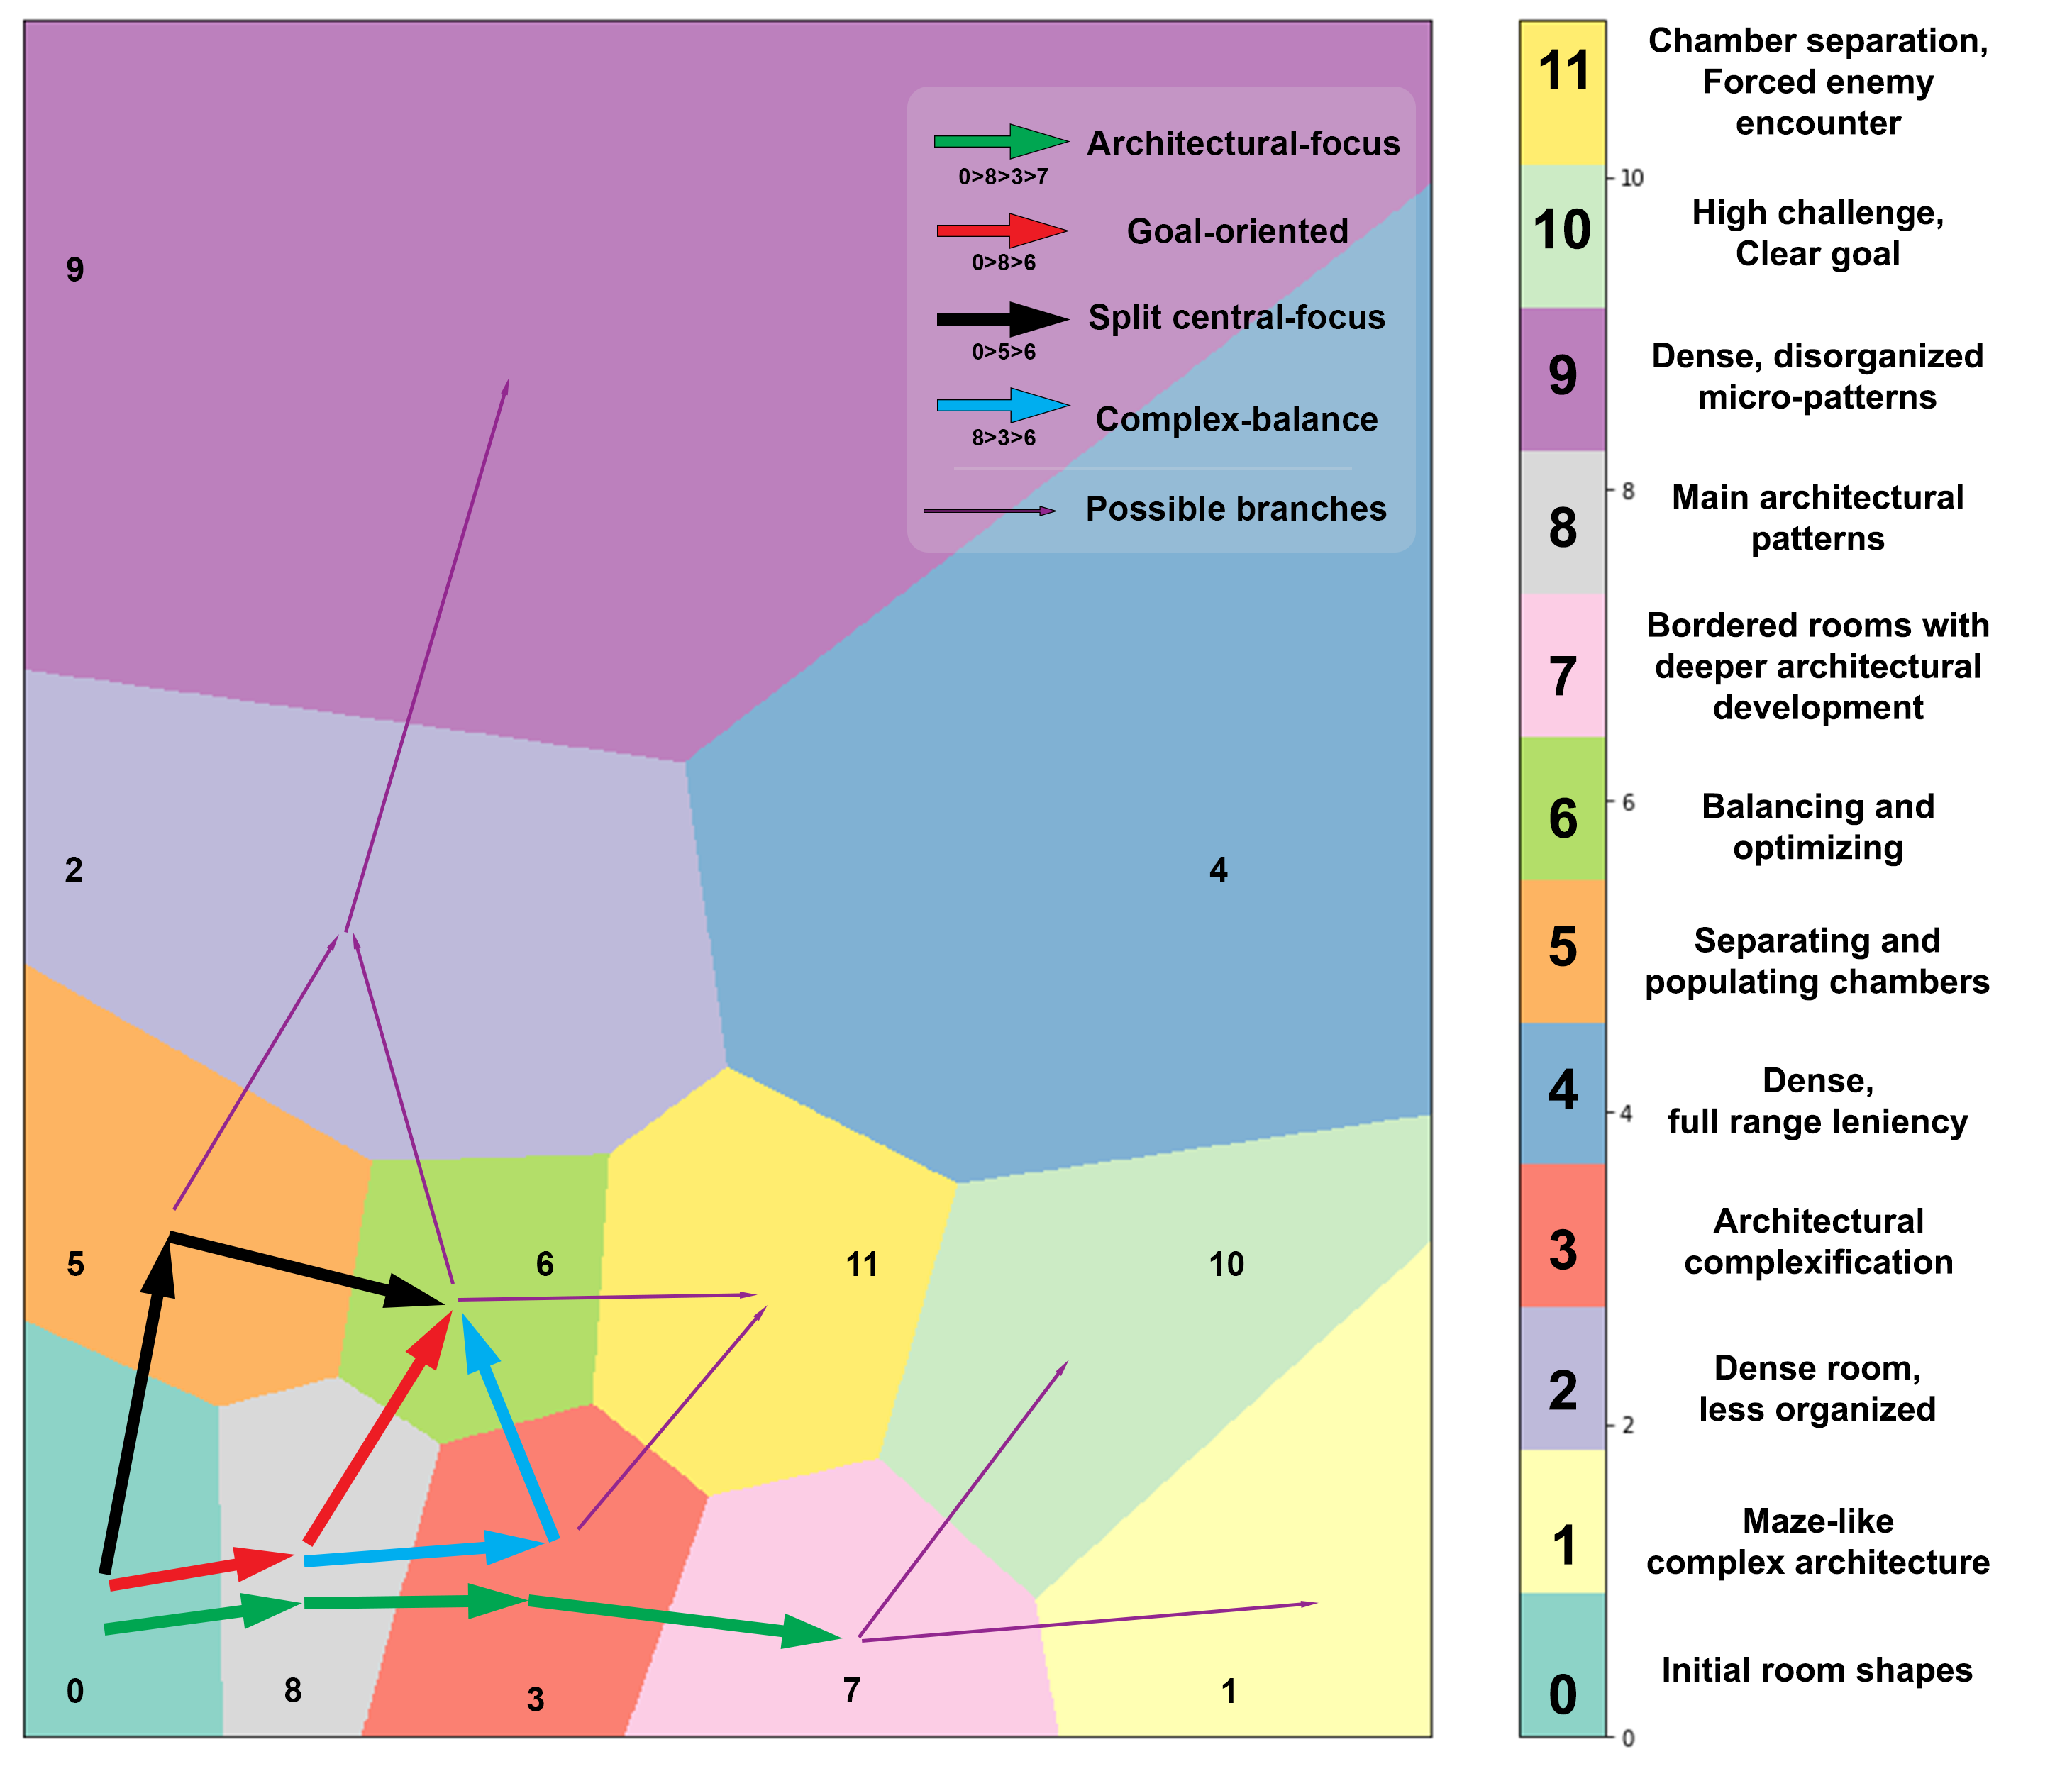
\includegraphics[width=\textwidth]{figures/resulting-paths-FINAL.png}}
\caption{Final and common designer trajectories. With thick arrows it is presented the archetypical paths, calculated using the frequencies of subsequences from $180$ diverse rooms. Each color represent a unique trajectory; with green the \textsc{Architectural-focus}, with red the \textsc{Goal-oriented}, with black the \textsc{Split central-focus}, and with blue the \textsc{Complex-balance}. Finally, thinner purple arrows extending from clusters traversed by the archetypical paths show the multiple possible branches that an archetypical path can deviate or extend to.} \label{p6fig:finalPaths}
\end{figure*}

% \begin{figure*}[t]
% \centerline{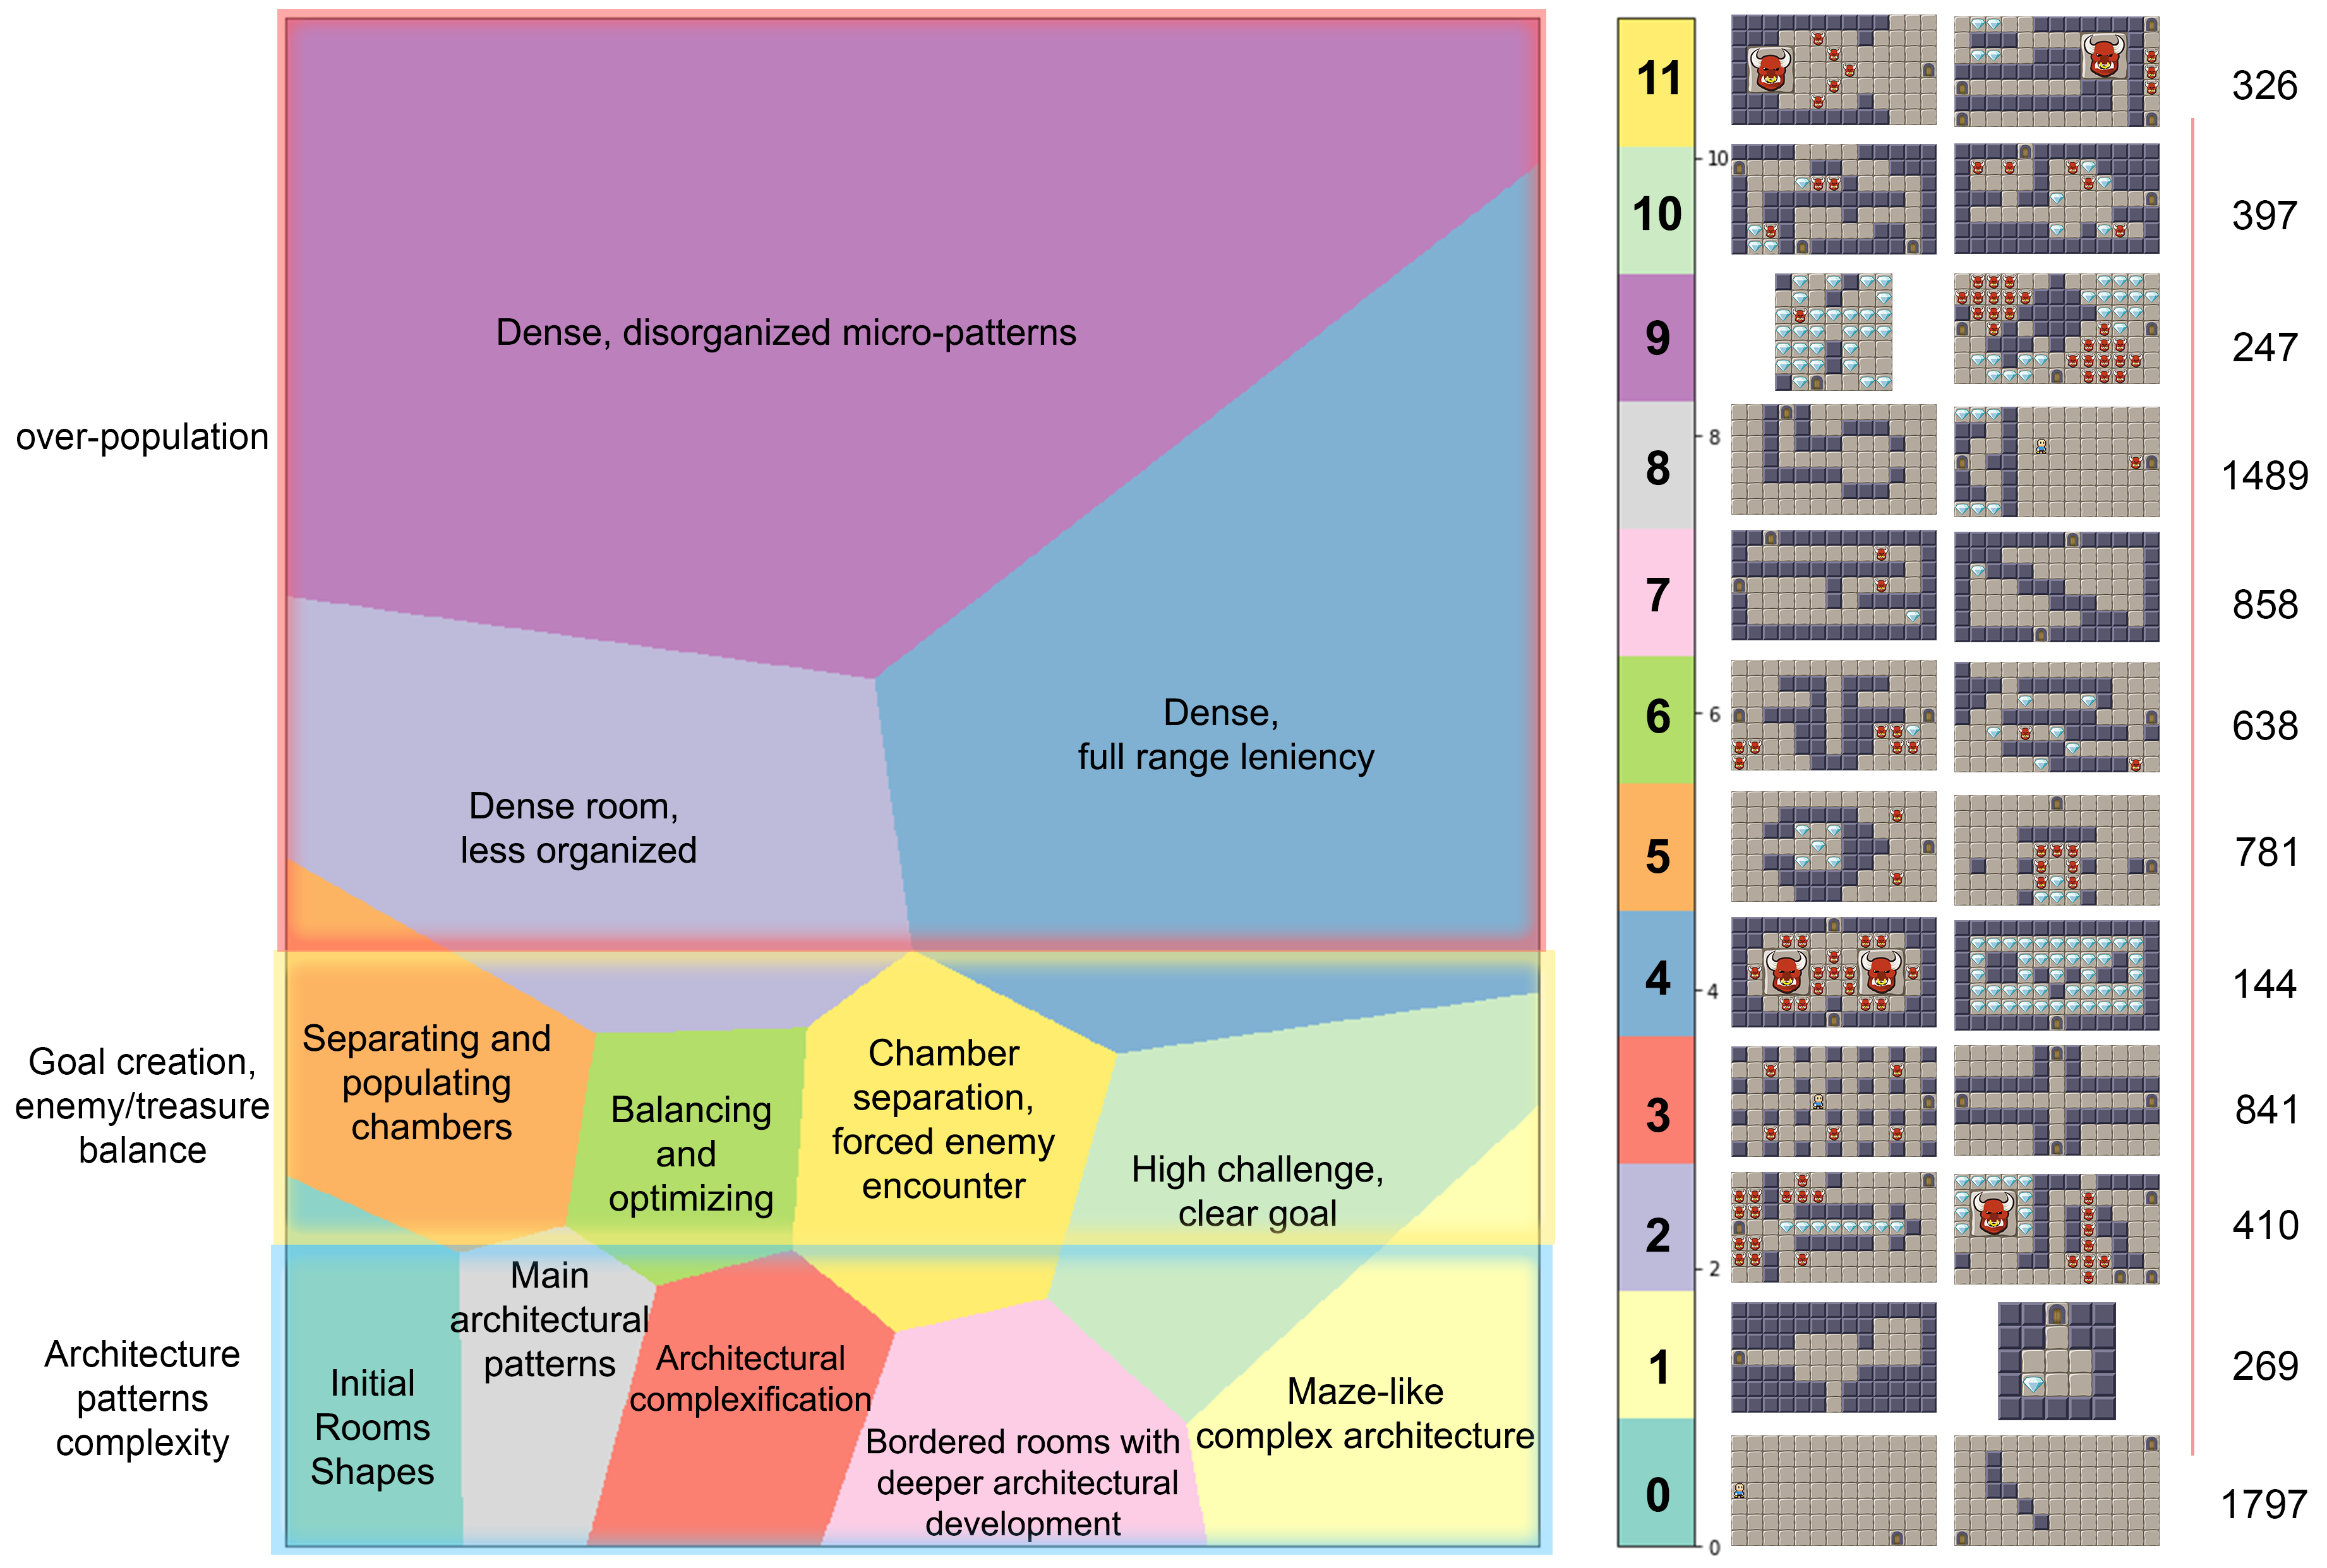
\includegraphics[width=16cm]{figures/final-cluster.png}}
% \caption{Best resulting cluster sets. (a) is K-Means (K=9), and (b) is K-Means (K=12), both are using the \textbf{Tiles} Dataset. While (b) performs slightly worst in the internal indices, when inspecting the qualitative features, it successfully subdivides the main bottom clusters which grants us with more granularity to label and cluster the design process of designers.} \label{p6fig:all-clusters}
% \end{figure*}

% \begin{figure}[t]
% \centerline{\includegraphics[width=8cm]{figures/cluster-figure-updated.png}}
% \caption{Overview of how the design style clustering would be used and integrated into the evaluation of the suggestions provided to the user. %is used and integrates into the evaluation of the suggestions provided to the user.
% } \label{p6fig:cluster}
% \end{figure}

% \begin{figure}[t]
% \centerline{\includegraphics[width=8cm]{figures/all_clusters.png}}
% \caption{All the selected clusters to be labeled and analyzed. In order, each of the clustering approaches correspond to the setups presented in table~\ref{p6table:setups}. (e) Shows extra information on the designs that were clustered together, and which were used to label the respective cluster.} \label{p6fig:all-clusters}
% \end{figure}

% \begin{figure}[b]
% \centerline{\includegraphics[width=8cm]{figures/hand-made-clusters.png}}
% \caption{Example of hand-made room designs used to create the clusters. only (a) and (b) belong to the same clusters} \label{p6fig:handMadeClustered}
% \end{figure}

% \begin{figure*}[t]
% \centerline{\includegraphics[width=18cm]{figures/approach_steps.png}}
% \caption{Rooms at generation $2090$ targeting Number of spatial-patterns (X) and Symmetry (Y). Each cell displays (top-right) the fitness of the optimal individual in its related feasible population. }
% \label{p6figs:approachSteps}
% \end{figure*}

% \begin{figure}[t]
% \centerline{\includegraphics[width=8cm]{figures/cluster-figure-updated.png}}
% \caption{Example of a figure caption.}
% \label{p6fig:implementationClusters}
% \end{figure}